Contents that are not used for the workshop paper

%We mostly do this and this in the customer service context - \cite{rapp2021human} \cite{jain2018evaluating}
%We don't yet know how to do that \cite{volkel2021eliciting} \cite{clark2019makes}

%Because of that, the act of implementation in the service industry, specifically in financial industry
%Useful for the industry, but leads to marginalization of the employees


%To ease this anxiety, some people hire professionals like financial advisors to manage their personal finances, while others are looking for digital capabilities to help them. Financial institutions are building online services to fulfill the needs of their customers and many of these institutions have heavily invested in conversational agents [2]. However, there is a paucity of research in design guidelines for conversational agents in financial services, both in the industry and academia. Also, existing research in financial services mostly focused on the customer service context to assist users with transactional inquiries, but did not look at how to use artificial agents to support users in their decision making process.


%Complex conversations - under-developed, leads to marginalization within those institutions that implement them
%Thus, we argue (the message to the CUI community) the development of more complex interactions (from SRI applications) including social interactions in addition to transaction ones are needed not just to diversify the potential of CUI, but also to address / mitigate issues of simple / straightfoward / transactional / easy to make CUIs.  Because of this, it is augmenting the "low value work" in financial employees (stay away from the use of replacement, use augmentation instead)

%The fact that we are not yet good at the more complex interactions - social interactions, we are predominantly developing simple interfaces, and that leads to inequalities at workplaces. Goal - let's work on making things more complex.

%Good connection to the conversation architecture paper - one of the components to build more complex interactions



%In addition to socio-economical marginalization, there are also perpetrating stereotypes - gender, culture

%We are mostly thinking about marginalization on the user side, but here we are looking at marginalization within the industry - not direct interaction with the users

%Marginalization of the workers as the CUIs represent these workers, how they affect work dynamics


%Growing income inequalities (Gini index shows more inequalities);
%people are not satisfied with their financial situation (US survey)
%Contributing to this is the access to financial services, a.k.a. financial inclusion
%Digital capabilities such as conversational agents contribute to this the gap in financial inclusion
%\url{https://research.aimultiple.com/conversational-banking/}


%State of CUIs and their design for marginalized and vulnerable populations. Existing research provides preliminary insights into the perceptions and barriers to CUI use for marginalized and vulnerable populations (e.g., on CUIs for older adults). What are the important opportunities, challenges, and open issues when it comes to CUI design for marginalized and vulnerable populations, such as older adults? Are there discrepancies between what was intended by CUI developers and what has been found in research (e.g., as hinted in previous research)? Is there evidence that some CUIs and their design unintentionally exclude different user groups, for example on the basis of age, race, or gender?

%For instance, there are large disparities in the availability and pricing of financial products (e.g. mortgage loans) across different demographic groups. \cite{dobbie2021measuring}.

%While digital solutions are providing easier access to some financial products and services, they are also reinforcing deep rooted inequalities within the financial industry. One of such inequalities is the practice of structuring access to financial products based on consumers' net worth. This is especially evident in the offering of private wealth solutions by large established financial institutions, providing dedicated and personalized services for high net worth individuals (e.g. BMO Private Wealth Services\footnote{https://www.bmo.com/privatewealth/services/}). These practices are also evident in new FinTech companies that are built on digital solutions, such as the robo-advisor company WealthSimple segregating their service offerings by net worth (\autoref{fig:ws_tieredservice}). These types of marginalizing practices are also evident in the conversational agents created by financial institutions.

\section{Digital Design Marginalization}

\begin{marginfigure}[-0pc]
  \begin{minipage}{\marginparwidth}
    \centering
    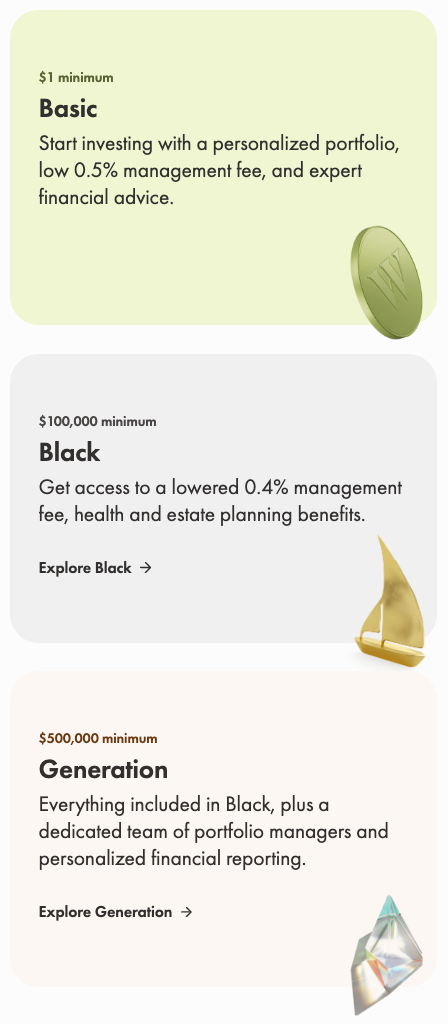
\includegraphics[width=0.9\marginparwidth]{figures/WealthSimple.png}
    \caption{WealthSimple: example of financial services segregated by net worth\footnote{https://www.wealthsimple.com/en-ca/invest/managed-investing}}
    \label{fig:ws_tieredservice}
  \end{minipage}
\end{marginfigure}

\begin{marginfigure}[-12pc]
  \begin{minipage}{\marginparwidth}
    \centering
    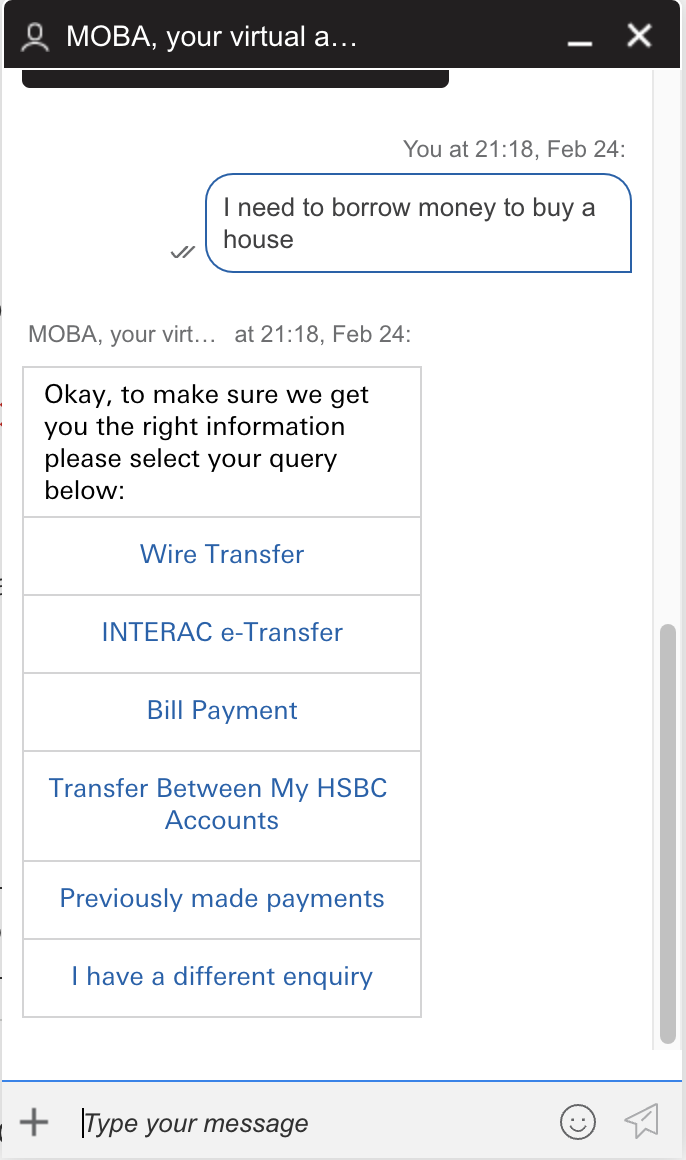
\includegraphics[width=0.9\marginparwidth]{figures/HSBC-goalbased.png}
    \caption{HSBC: Inquiries based on personal goals was not interpreted correctly}
    \label{fig:hsbc-goalbased}
  \end{minipage}
\end{marginfigure}

\begin{marginfigure}[1pc]
  \begin{minipage}{\marginparwidth}
    \centering
    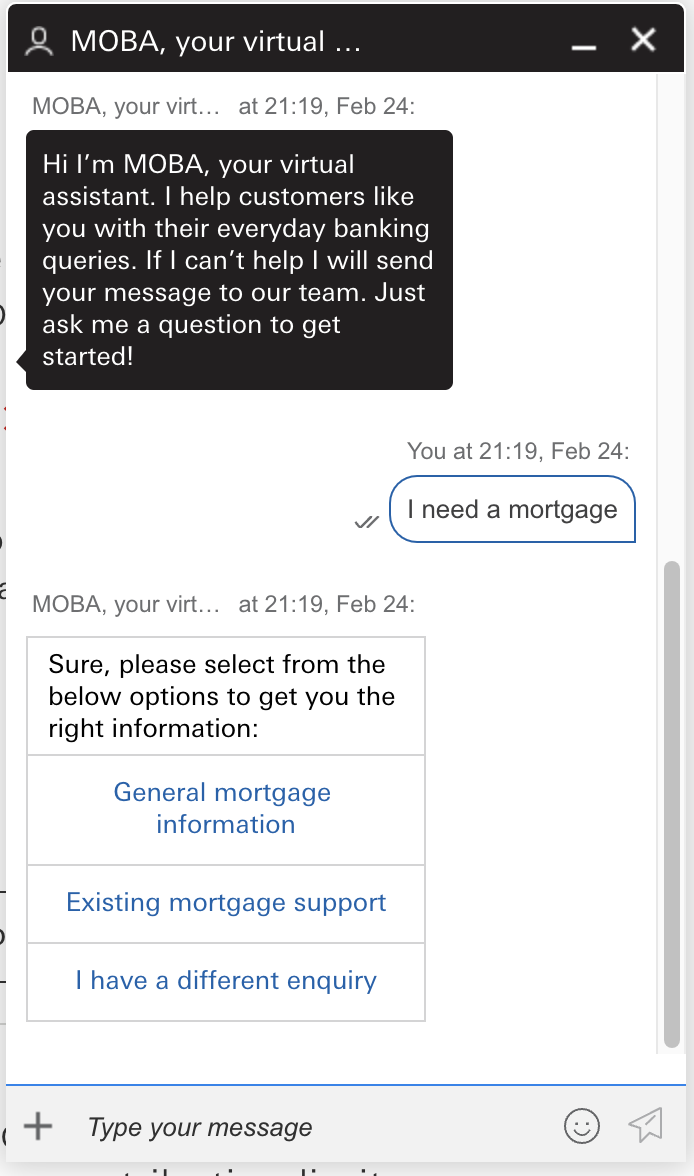
\includegraphics[width=0.9\marginparwidth]{figures/HSBC-productbased.png}
    \caption{HSBC: Inquiries based on financial product terms was interpreted correctly}
    \label{fig:hsbc-productbased}
  \end{minipage}
\end{marginfigure}

Sin et al \cite{sin2021digital} defined Digital Design Marginalization (DDM) as the pushing of a defined group of users away from a digital or online service or system. Specifically for conversational agents, three different perspectives of DDM are discussed below: limited access to end consumers, assumptions about financial and digital literacy, and marginalization through success measures.

First aspect of DDM is related to the limited access financial institutions have to their end customers. Financial institutions may not have direct relationships with their end customers for certain financial products as they are offered through an intermediary model. For example, financial advisors as an intermediaries are purchasing mutual funds from financial institutions on behalf of their clients. As a result, financial institutions do not have direct relationships with their end customers and need to rely on intermediaries to understand their needs. In essence, the intermediaries are acting as proxies to represent the needs of their clients. This is prone to issues of misrepresentation of information, as there are misaligned incentives between the intermediaries and their clients. For example, a financial advisor wanting to attract younger clients may work with financial institutions to design virtual agents to help with topics such as paying off student loans, while ignoring their retired clients' needs for resources to manage the decumulation of their capital.

There are also design marginalization within the financial institutions themselves. In large financial institutions, the success of digital initiatives such as building a new conversational agent would be evaluated by measures such as adoption statistics (e.g. usage per day), user satisfaction (e.g. net promoter score), and cost savings (e.g. call reduction into service centers). These quantitative measures create the incentive to focus on mass adoption in a short amount of time, potentially leaving out the needs of the vulnerable populations. For example, it is easier to achieve better success measures to build features for those who are already using the digital tools, instead of investing in resources to help customers who are not currently using the digital tools to learn how to use them.

Lastly, there is a fundamental mismatch between financial institutions' information organization and users' mental model about financial products. Users generally approach their financial needs based on their personal goals, such as buying a house. After realizing their goals, then they would work to identify the financial need and suitable financial products to achieve those goals. However, most financial conversational agents are designed to discuss specific financial products instead of matching users goals with these products. This means it is up to the user to match their personal goals to financial products, which requires a certain level of financial literacy. In the case above to borrow money to buy a house, potentially suitable financial products can be a loan, line of credit, or mortgage. As you can see from \autoref{fig:hsbc-goalbased}, the HSBC chatbot does not understand the inquiry based on personal goals to borrow money, but was able to recognized questions related to specific financial products like mortgages (\autoref{fig:hsbc-productbased}). This means that the convenience of using a conversational agent does not help individuals who cannot speak the language of the financial institutions in their terms. %In addition to discrimination against financial literacy, there is also the overall segregation to the access of product that exist in the industry.





%A project’s success is measured on . This creates the incentive to focus on mass adoption in a short amount of time, potentially leaving out the needs of the minority vulnerable populations. For example, those who are laid off from an employer may be in financial hardship and can benefit from taking out an emergency loan from their retirement plan. However, they would not be able to access the virtual assistant for help, as they do not have access to the digital infrastructure anymore after being laid off.  Their only option is to call in for assistance, limiting their choices in a dire situation. Also, a company’s financial incentives may be at odds with inclusive design. For example, a company may not want participants to withdraw large amounts digitally, as this will impact the company’s financial performance. Instead, these large sum transactions can only be done by calling into the service center to discuss with a human representative. This design choice is potentially marginalizing, especially in situations where large sums of money is needed for emergency situations. If the needs of the minority marginalized population can be made aware by decision makers in the boardroom instead of assessing purely on statistics, it will help to bridge the gap for inclusive design.


%\textbf{Misaligned incentives:}
%The financial world is tangled web of different stakeholders with different objectives. For example, as a financial institution offering retirement plans, their direct beneficiaries are the plan participants who are the employees receiving the retirement benefits. However, the main stakeholder works with is the plan sponsor, of the company that is offering the retirement plan to their employees. There are also other intermediaries, such as financial advisors who help plan sponsors choose a retirement plan. These stakeholders have different incentives: plan sponsors wants to highlight the value of the retirement plan to their employees but also want to reduce expenses on these plans; financial advisors are looking to earn commissions on matching to the retirement plans while adhering to their fiduciary duties; and the plan participants are looking to maximize their retirement savings. While financial institutions should be focused on providing the best services to plan participants, their decisions are usually swayed by the other key stakeholders who are the ones paying for the services. As such, their incentives usually creep into the digital products they offer. One example is to use conversational agents to highlight the benefits the employer is providing, or to nudge them towards cost-saving measures instead of actually maximizing their savings.

%\textbf{No easy access to end-users:}
%Also, within the world of intermediaries in financial services, it is difficult to get access to the end users who are benefiting from the services as they are controlled by the intermediaries. As such, the intermediaries are searching as proxies to voice the opinions of their customers. However, it could lead to mismatches either due to a lack of understanding, or potentially malicious means to maximize their own gains instead. Without direct access to the end customers, it is very difficult to design digital solutions such as conversational agents that are solving for user needs.

%There may be capabilities that the intermediaries are deliberately hiding from their customers. For example, different licenses are required to work with different financial products in Canada. For example, a MGA license is required to sell insurance, while an IIROC license is required to sell mutual funds or individual stocks. For an advisor who is only MGA license who do not have an IIROC license, they may be incentivized to advertise market-linked insurance products like segregated funds to their customers, instead of admitting to their limitations of not able to provide advice of mutual fund products. This bias can also be reflected in digital solutions like conversational agents. For example, a conversational agent representing a firm that can only has the license to sell insurance products may recommend different insurance-based products to the client, but does not mention other possibilities like index funds or mutual funds. This is also the same for companies that only provide recommendations within their own offerings.

%A project’s success is measured on adoption statistics (e.g. usage per day), user satisfaction (e.g. net promoter score), and cost savings (e.g. call reduction into call center). This creates the incentive to focus on mass adoption in a short amount of time, potentially leaving out the needs of the minority vulnerable populations. For example, those who are laid off from an employer may be in financial hardship and can benefit from taking out an emergency loan from their retirement plan. However, they would not be able to access the virtual assistant for help, as they do not have access to the digital infrastructure anymore after being laid off.  Their only option is to call in for assistance, limiting their choices in a dire situation. Also, a company’s financial incentives may be at odds with inclusive design. For example, a company may not want participants to withdraw large amounts digitally, as this will impact the company’s financial performance. Instead, these large sum transactions can only be done by calling into the service center to discuss with a human representative. This design choice is potentially marginalizing, especially in situations where large sums of money is needed for emergency situations. If the needs of the minority marginalized population can be made aware by decision makers in the boardroom instead of assessing purely on statistics, it will help to bridge the gap for inclusive design.

%\textbf{Assumptions about Financial Literacy: }
%There is a fundamental mismatch between financial institutions' information organization and users' mental model about financial products. Users generally approach their financial needs based on their personal goals, such as buying a house. After realizing their goals, then they would work to identify the financial need and suitable financial products to achieve those goals. However, most financial conversational agents are designed to discuss specific financial products instead of matching users goals with these products. This means it is up to the user to match their personal goals to financial products, which requires a certain level of financial literacy. In the case above to borrow money to buy a house, potentially suitable financial products can be a loan, line of credit, or mortgage. As you can see from \autoref{fig:hsbc}, using the common language asking HSBC chatbot to borrow money was not understood, but asking for specific financial product, mortgage, was recognized. This means that the convenience of using a conversational agent does not help individuals who cannot speak the language of the financial institutions in their terms. In addition to discrimination against financial literacy, there is also the overall segregation to the access of product that exist in the industry.

%Within large financial institutions, they usually operate as separate lines of businesses, such as personal banking (e.g. bank accounts, credit cards), investing (e.g. mutual funds, stocks), and insurance products. This segregation is reflected in the digital world, in both websites and by extension to conversational agents. For CAs helping users with their specific financial needs, usually they need to authenticated in order to provide detailed access to the clients' accounts. However, given the segregation of lines of business, most financial institutions have different authenticated sites for different parts of their businesses. For example someone with an insurance product and a bank account may have different  sites to log in to access their products. Usually conversational agents are built behind these firewalls and can only service the lines of business that they exist in, with no information shared across different accounts. This leads to information silo for the users, which may lead to suboptimal decisions. For example, a user needs a sum of money for emergency repair at home. Technically there are choices from their bank account overdraft, credit card, loans, and insurance withdraws. However, given the segregation between lines of businesses, a user is not able to find resources to compare across the financial products within the same financial institution. This segregation between lines of business also leads to other issues such as privacy of data.


\section{Privacy}


As conversational agents use natural speech, there is the potential to share personal and confidential data with parties that are not entitled to that information. As mentioned above, there are segregation between lines of businesses, where by regulation or organization construct, each line of business can only discuss the financial products within their domain. However, users usually do not understand the differences in lines of businesses as defined by financial institutions and may be sharing personal data that the counterparty does not have privilege to know. This already happens within in-person customer services, and it is also happening digitally. This is exasperated by the natural format of conversational agents, as users feel like they can discuss products within the same financial institution with the conversational agents, and do not understand the privacy issues across lines of businesses.

To combat this privacy issue, some companies choose to implement for strict conversation structure, such as a decision tree where there is no user input, but the user is choosing between different preset options. While this approach helps with the sharing of unintended private information, it is taking away from the naturalness of the conversation, making it less useful to implement in a conversational format.


\section{ACM Copyrights \& Permission Policy}
Accepted extended abstracts and papers will be distributed in the
Conference Publications. They will also be placed in the ACM Digital
Library, where they will remain accessible to thousands of researchers
and practitioners worldwide. To view the ACM's copyright and
permissions policy, see:
\url{http://www.acm.org/publications/policies/copyright_policy}.

%\marginpar{%
%  \vspace{-45pt} \fbox{%
%    \begin{minipage}{0.925\marginparwidth}
%      \textbf{Good Utilization of the Side Bar} \\
%      \vspace{1pc} \textbf{Preparation:} Do not change the margin
%      dimensions and do not flow the margin text to the
%      next page. \\
%      \vspace{1pc} \textbf{Materials:} The margin box must not intrude
%      or overflow into the header or the footer, or the gutter space
%      between the margin paragraph and the main left column. The text
%      in this text box should remain the same size as the body
%      text. Use the \texttt{{\textbackslash}vspace{}} command to set
%      the margin
%      note's position. \\
%      \vspace{1pc} \textbf{Images \& Figures:} Practically anything
%      can be put in the margin if it fits. Use the
%      \texttt{{\textbackslash}marginparwidth} constant to set the
%      width of the figure, table, minipage, or whatever you are trying
%      to fit in this skinny space.
%    \end{minipage}}\label{sec:sidebar} }

\section{Page Size}
All SIGCHI submissions should be US letter (8.5 $\times$ 11
inches). US Letter is the standard option used by this \LaTeX\
template.

\section{Text Formatting}
Please use an 8.5-point Verdana font, or other sans serifs font as
close as possible in appearance to Verdana in which these guidelines
have been set. Arial 9-point font is a reasonable substitute for
Verdana as it has a similar x-height. Please use serif or
non-proportional fonts only for special purposes, such as
distinguishing \texttt{source code} text.

\subsubsection{Text styles}
The \LaTeX\ template facilitates text formatting for normal (for body
text); heading 1, heading 2, heading 3; bullet list; numbered list;
caption; annotation (for notes in the narrow left margin); and
references (for bibliographic entries). Additionally, here is an
example of footnoted\footnote{Use footnotes sparingly, if at all.}
text. As stated in the footnote, footnotes should rarely be used.

\begin{figure}
  \includegraphics[width=0.9\columnwidth]{figures/sigchi-logo}
  \caption{Insert a caption below each figure.}~\label{fig:sample}
\end{figure}

\subsection{Language, style, and content}
The written and spoken language of SIGCHI is English. Spelling and
punctuation may use any dialect of English (e.g., British, Canadian,
US, etc.) provided this is done consistently. Hyphenation is
optional. To ensure suitability for an international audience, please
pay attention to the following:

\begin{table}
  \centering
  \begin{tabular}{l r r r}
    % \toprule
    & & \multicolumn{2}{c}{\small{\textbf{Test Conditions}}} \\
    \cmidrule(r){3-4}
    {\small\textit{Name}}
    & {\small \textit{First}}
      & {\small \textit{Second}}
    & {\small \textit{Final}} \\
    \midrule
    Marsden & 223.0 & 44 & 432,321 \\
    Nass & 22.2 & 16 & 234,333 \\
    Borriello & 22.9 & 11 & 93,123 \\
    Karat & 34.9 & 2200 & 103,322 \\
    % \bottomrule
  \end{tabular}
  \caption{Table captions should be placed below the table. We
    recommend table lines be 1 point, 25\% black. Minimize use of
    table grid lines.}~\label{tab:table1}
\end{table}

\begin{itemize}\compresslist%
\item Write in a straightforward style. Use simple sentence
  structure. Try to avoid long sentences and complex sentence
  structures. Use semicolons carefully.
\item Use common and basic vocabulary (e.g., use the word ``unusual''
  rather than the word ``arcane'').
\item Briefly define or explain all technical terms. The terminology
  common to your practice/discipline may be different in other design
  practices/disciplines.
\item Spell out all acronyms the first time they are used in your
  text. For example, ``World Wide Web (WWW)''.
\item Explain local references (e.g., not everyone knows all city
  names in a particular country).
\item Explain ``insider'' comments. Ensure that your whole audience
  understands any reference whose meaning you do not describe (e.g.,
  do not assume that everyone has used a Macintosh or a particular
  application).
\item Explain colloquial language and puns. Understanding phrases like
  ``red herring'' requires a cultural knowledge of English. Humor and
  irony are difficult to translate.
\item Use unambiguous forms for culturally localized concepts, such as
  times, dates, currencies, and numbers (e.g., ``1-5- 97'' or
  ``5/1/97'' may mean 5 January or 1 May, and ``seven o'clock'' may
  mean 7:00 am or 19:00). For currencies, indicate equivalences:
  ``Participants were paid {\fontfamily{txr}\selectfont \textwon}
  25,000, or roughly US \$22.''
\item Be careful with the use of gender-specific pronouns (he, she)
  and other gender-specific words (chairman, manpower,
  man-months). Use inclusive language (e.g., she or he, they, chair,
  staff, staff-hours, person-years) that is gender-neutral. If
  necessary, you may be able to use ``he'' and ``she'' in alternating
  sentences, so that the two genders occur equally
  often~\cite{Schwartz:1995:GBF}.
\item If possible, use the full (extended) alphabetic character set
  for names of persons, institutions, and places (e.g.,
  Gr{\o}nb{\ae}k, Lafreni\'ere, S\'anchez, Nguy{\~{\^{e}}}n,
  Universit{\"a}t, Wei{\ss}enbach, Z{\"u}llighoven, \r{A}rhus, etc.).
  These characters are already included in most versions and variants
  of Times, Helvetica, and Arial fonts.
\end{itemize}

% \begin{figure}
%   \includegraphics[width=.9\columnwidth]{figures/ea-figure2}
%   \caption{If your figure has a light background, you can set its
%     outline to light gray, like this, to make a box around
%     it.}\label{fig:bats}
% \end{figure}

\begin{marginfigure}[-35pc]
  \begin{minipage}{\marginparwidth}
    \centering
    \includegraphics[width=0.9\marginparwidth]{figures/cats}
    \caption{In this image, the cats are tessellated within a square
      frame. Images should also have captions and be within the
      boundaries of the sidebar on page~\pageref{sec:sidebar}. Photo:
      \cczero~jofish on Flickr.}~\label{fig:marginfig}
  \end{minipage}
\end{marginfigure}

\section{Figures}
The examples on this and following pages should help you get a feel
for how screen-shots and other figures should be placed in the
template. Your document may use color figures (see
Figures~\ref{fig:sample}), which are included in the page limit; the
figures must be usable when printed in black and white. You can use
the \texttt{\marginpar} command to insert figures in the (left) margin
of the document (see Figure~\ref{fig:marginfig}). Finally, be sure to
make images large enough so the important details are legible and
clear (see Figure~\ref{fig:cats}).
All figures should include alt text (figure description) for improved accessibility – see the Accessibility section.

\section{Tables}
You man use tables inline with the text (see Table~\ref{tab:table1})
or within the margin as shown in Table~\ref{tab:table2}. Try to
minimize the use of lines (especially vertical lines). \LaTeX\ will
set the table font and captions sizes correctly; the latter must
remain unchanged.

\section{Accessibility}
The Executive Council of SIGCHI has committed to making SIGCHI
conferences more inclusive for researchers, practitioners, and
educators with disabilities. As a part of this goal, the all authors
are expected to work on improving the accessibility of their
submissions. Specifically, we encourage authors to carry out the
following five steps:
\begin{itemize}\compresslist%
\item Add alternative text (figure description) to all figures
\item Mark table headings
\item Generate a tagged PDF
\item Verify the default language
\item Set the tab order to ``Use Document Structure''
\end{itemize}

For links to detailed instructions and resources, please see:
\url{http://chi2020.acm.org/authors/papers/guide-to-an-accessible-submission/}

Unfortunately good tools do not yet exist to create tagged PDF files
from Latex. \LaTeX\ users will need to carry out all of the above
steps in the PDF directly using Adobe Acrobat, after the PDF has been
generated.


\begin{figure*}
  \centering
  \includegraphics[width=1.3\columnwidth]{figures/map}
  \caption{In this image, the map maximizes use of space. You can make
    figures as wide as you need, up to a maximum of the full width of
    both columns. Note that \LaTeX\ tends to render large figures on a
    dedicated page. Image: \ccbynd~ayman on Flickr.}~\label{fig:cats}
\end{figure*}

\section{Producing and Testing PDF Files}
We recommend that you produce a PDF version of your submission well
before the final deadline.

\marginpar{\vspace{-23pc}So long as you don't type outside the right
  margin or bleed into the gutter, it's okay to put annotations over
  here on the left, too; this annotation is near Hawaii. You'll have
  to manually align the margin paragraphs to your \LaTeX\ floats using
  the \texttt{{\textbackslash}vspace{}} command.}

\begin{margintable}[1pc]
  \begin{minipage}{\marginparwidth}
    \centering
    \begin{tabular}{r r l}
      & {\small \textbf{First}}
      & {\small \textbf{Location}} \\
      \toprule
      Child & 22.5 & Melbourne \\
      Adult & 22.0 & Bogot\'a \\
      \midrule
      Gene & 22.0 & Palo Alto \\
      John & 34.5 & Minneapolis \\
      \bottomrule
    \end{tabular}
    \caption{A simple narrow table in the left margin
      space.}~\label{tab:table2}
  \end{minipage}
\end{margintable}
Test your PDF file by viewing or printing it with the same software we
will use when we receive it, Adobe Acrobat Reader Version 10. This is
widely available at no cost. Note that most
reviewers will use a North American/European version of Acrobat
reader, so please check your PDF accordingly.

\section{Acknowledgements}
We thank all the volunteers, publications support, staff, and authors
who wrote and provided helpful comments on previous versions of this
document. As well authors 1, 2, and 3 gratefully acknowledge the grant
from NSF (\#1234--2222--ABC). Author 4 for example may want to
acknowledge a supervisor/manager from their original employer. This
whole paragraph is just for example. Some of the references cited in
this paper are included for illustrative purposes only.

\section{References Format}
Your references should be published materials accessible to the
public. Internal technical reports may be cited only if they are
easily accessible and may be obtained by any reader for a nominal
fee. Proprietary information may not be cited. Private communications
should be acknowledged in the main text, not referenced (e.g.,
[Golovchinsky, personal communication]). References must be the same
font size as other body text. References should be in alphabetical
order by last name of first author. Use a numbered list of references
at the end of the article, ordered alphabetically by last name of
first author, and referenced by numbers in brackets. For papers from
conference proceedings, include the title of the paper and the name of
the conference. Do not include the location of the conference or the
exact date; do include the page numbers if available. 

References should be in ACM citation format:
\url{http://www.acm.org/publications/submissions/latex_style}.  This
includes citations to Internet
resources~\cite{CHINOSAUR:venue,cavender:writing,psy:gangnam}
according to ACM format, although it is often appropriate to include
URLs directly in the text, as above. Example reference formatting for
individual journal articles~\cite{ethics}, articles in conference
proceedings~\cite{Klemmer:2002:WSC:503376.503378},
books~\cite{Schwartz:1995:GBF}, theses~\cite{sutherland:sketchpad},
book chapters~\cite{winner:politics}, an entire journal
issue~\cite{kaye:puc},
websites~\cite{acm_categories,cavender:writing},
tweets~\cite{CHINOSAUR:venue}, patents~\cite{heilig:sensorama}, 
games~\cite{supermetroid:snes}, and
online videos~\cite{psy:gangnam} is given here.  See the examples of
citations at the end of this document and in the accompanying
\texttt{BibTeX} document. This formatting is a edited version of the
format automatically generated by the ACM Digital Library
(\url{http://dl.acm.org}) as ``ACM Ref''. DOI and/or URL links are
optional but encouraged as are full first names. Note that the
Hyperlink style used throughout this document uses blue links;
however, URLs in the references section may optionally appear in
black.